\scanpage{242}

-- \mspage{16} -- \hfill n° 227

3. \uline{L'application rationnelle définie par un système linéaire}.

On continue à supposer $V$ complète. Soit $\mathcal L$ un système linéaire, $X_0\in\mathcal L$, et $L_0$ le module dérivé de $\mathcal L$ par $X_0$. Soit $f_0,\ldots,f_n$ une base de ce module. Alors les fonctions $(1,f_1/f_0,\ldots,f_n/f_0)$ peuvent être prises comme coordonnées non homogènes d'un point dans l'espace projectif, qui représente un point générique d'une variété projective $V'$. Si $t$ est un élément transcendant sur tout, alors $(tf_0,\ldots,tf_n)$ sont les coordonnées homogènes d'un point générique de $V'$. Elles définissent une application rationnelle $T:V\longrightarrow V'$ de $V$ sur $V'$. Un changement de base dans $L_0$ donne une transformation projective de $V'$.

Si on employait un module $L_1$ dérivé de $\mathcal L$ par un autre diviseur $X_1$, on voit que l'application rationnelle $T_1$ obtenue comme ci-dessus diffère de $T$ par une transformation \deleted{linéaire}\inserted{projective}. On peut donc dire que $T$ est uniquement déterminée par $\mathcal L$. De plus, si $\mathcal L$ et $\mathcal L'$ soit deux systèmes linéaires qui ne diffèrent que par une composante fixe, alors on voit immédiatement qu'ils donnent lieu à la même application rationnelle $T$ de $V$, les modules dérivés étant les mêmes. Pour étudier l'application rationnelle associée à un système linéaire, on peut donc se borner, sans perte de généralité, aux systèmes linéaires \unsure{sans'|sans} composantes fixes.

\figure{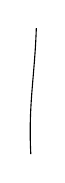
\begin{tikzpicture}[x=1cm,y=1cm]
\draw (0.07,1.6) to[out=-92,in=93] (0,0);
\end{tikzpicture}}

On va maintenant donner un critère pour que l'application rationnelle $T$ soit définie en un point $P$ de $V$.

Un point $P$ de $V$ est dit un \uline{point de base} du système linéaire $\mathcal L$ si $P\in\inserted{\unsure{\checkmark|\gamma}}|X|$ pour tout $X\in\mathcal L$. Si $Y$ est une composante fixe de $\mathcal L$, alors tous les points de $|Y|$ sont des points de base. Il peut très bien arriver qu'un système linéaire n'ait pas de composante fixe, mais ait

\mspage{241}
